\documentclass{article}
\usepackage{graphicx}
\usepackage{wrapfig}
\usepackage{filecontents}
\usepackage{siunitx}
\usepackage[table]{xcolor}
\usepackage{float}
\usepackage{hyperref}

\usepackage{color} % balíček pro obarvování textů
\usepackage{xcolor}  % zapne možnost používání barev, mj. pro \definecolor
\usepackage{pgfplots} % http://www.chiark.greenend.org.uk/doc/texlive-doc/latex/pgfplots/pgfplots.pdf

\ifnum 0\ifxetex 1\fi\ifluatex 1\fi=0 % if pdftex
  \usepackage[T1]{fontenc}
  \usepackage[utf8]{inputenc}
\else % if luatex or xelatex
  \ifxetex
    \usepackage{mathspec}
  \else
    \usepackage{fontspec}
  \fi
  \defaultfontfeatures{Ligatures=TeX,Scale=MatchLowercase}
\fi
\usepackage[total={175mm,230mm}, top=23mm, left=20mm, includefoot]{geometry}
\hypersetup{
    colorlinks,
    linkcolor={blue!50!black},
    citecolor={green!50!black},
    urlcolor={blue!80!black}
}
% \definecolor{fialova}{RGB}{ 255, 000, 255}
\definecolor{color-si1}{RGB}{ 255, 000, 000}
\definecolor{color-si2}{RGB}{ 251, 130, 032}

\definecolor{color-ge1}{RGB}{ 000, 255, 000}
\definecolor{color-ge2}{RGB}{ 032, 251, 160}

\definecolor{color-inp1}{RGB}{ 000, 000, 255}
\definecolor{color-inp2}{RGB}{ 160, 032, 251}

\definecolor{color-geas1}{RGB}{ 225, 225, 000}
\definecolor{color-geas2}{RGB}{ 225, 225, 100}

\definecolor{sedak}{RGB}{ 100, 100, 100}


\newcommand \obr[1]
{ obr.~\ref{#1}}

\newcommand \tab[1]
{ tab.~ß\ref{#1}}


\begin{document}
\pagestyle{empty}

\definecolor{color_29791}{rgb}{0,0,0}
\begin{figure}[H]
    \hspace{-13mm}
    \begin{minipage}[t]{\textwidth}
        \vspace{-20mm}
        \begin{tikzpicture}[overlay]
            \path(0pt,0pt);
        \end{tikzpicture}
        \begin{picture}(-5,0)(2.5,0)
            \put(123.656,-82.75397){\fontsize{18}{1}\usefont{T1}{ptm}{m}{n}\selectfont\color{color_29791}VYSOKÉ UČENÍ TECHNICKÉ V BRNĚ}
            \put(76.296,-104.785){\fontsize{13}{1}\usefont{T1}{ptm}{m}{n}\selectfont\color{color_29791}FAKULTA  ELEKTROTECHNIKY A KOMUNIKAČNÍCH TECHNOLOGIÍ}
            \put(198.447,-128.5339){\fontsize{16}{1}\usefont{T1}{cmr}{b}{n}\selectfont\color{color_29791}Ústav elektrotechnologie}
            \put(156.848,-278.1589){\fontsize{14}{1}\usefont{T1}{ptm}{m}{n}\selectfont\color{color_29791}LABORATORNÍ CVIČENÍ Z PŘEDMĚTU}
            \put(83.123,-300.2579){\fontsize{14}{1}\usefont{T1}{cmr}{b}{n}\selectfont\color{color_29791}ELEKTROTECHNICKÉ MATERIÁLY A VÝROBNÍ PROCESY}
            \put(55.85,-421.25){\fontsize{14}{1}\usefont{T1}{cmr}{b}{n}\selectfont\color{color_29791}Číslo úlohy: 6}
            \put(55.85,-469.547){\fontsize{14}{1}\usefont{T1}{cmr}{b}{n}\selectfont\color{color_29791}Název úlohy: Počítačové vytváření pásových modelů polovodičových materiálů}
            \put(23.9,-620.32){\fontsize{12}{1}\usefont{T1}{cmr}{b}{n}\selectfont\color{color_29791}Jméno a příjmení, ID:}
            \put(23.9,-637.119){\fontsize{12}{1}\usefont{T1}{cmr}{b}{n}\selectfont\color{color_29791}Tomáš Vavrinec, 240893}
            \put(186.95,-620.32){\fontsize{12}{1}\usefont{T1}{cmr}{b}{n}\selectfont\color{color_29791}Atmosférický tlak:}
            \put(186.95,-637.119){\fontsize{12}{1}\usefont{T1}{cmr}{b}{n}\selectfont\color{color_29791}102.6 hPa}
            \put(293.25,-620.32){\fontsize{12}{1}\usefont{T1}{cmr}{b}{n}\selectfont\color{color_29791}Teplota okolí: }
            \put(293.25,-637.119){\fontsize{12}{1}\usefont{T1}{cmr}{b}{n}\selectfont\color{color_29791}25.1°C}
            \put(417.25,-620.32){\fontsize{12}{1}\usefont{T1}{cmr}{b}{n}\selectfont\color{color_29791}Relativní vlhkost:}
            \put(417.25,-637.119){\fontsize{12}{1}\usefont{T1}{cmr}{b}{n}\selectfont\color{color_29791}37.2\%}
            \put(23.9,-665.77){\fontsize{12}{1}\usefont{T1}{cmr}{b}{n}\selectfont\color{color_29791}Měřeno dne:}
            \put(23.9,-682.569){\fontsize{12}{1}\usefont{T1}{cmr}{b}{n}\selectfont\color{color_29791}14.10.2022}
            \put(186.95,-665.77){\fontsize{12}{1}\usefont{T1}{cmr}{b}{n}\selectfont\color{color_29791}Odevzdáno dne:}
            \put(293.25,-665.77){\fontsize{12}{1}\usefont{T1}{cmr}{b}{n}\selectfont\color{color_29791}Ročník, stud. skupina:}
            \put(293.25,-682.569){\fontsize{12}{1}\usefont{T1}{cmr}{b}{n}\selectfont\color{color_29791}2}
            \put(417.25,-665.77){\fontsize{12}{1}\usefont{T1}{cmr}{b}{n}\selectfont\color{color_29791}Kontrola:}
            \put(23.9,-703.42){\fontsize{12}{1}\usefont{T1}{cmr}{b}{n}\selectfont\color{color_29791}Spolupracovali:}
            \put(23.9,-720.219){\fontsize{12}{1}\usefont{T1}{cmr}{b}{n}\selectfont\color{color_29791}Daniel Poisl}
        \end{picture}
        \begin{tikzpicture}[overlay]
            \path(0pt,0pt);
            \draw[color_29791,line width=0.5pt]
            (20.4pt, -606.117pt) -- (20.4pt, -722.815pt)
            ;
            \draw[color_29791,line width=0.5pt]
            (183.45pt, -606.117pt) -- (183.45pt, -651.067pt)
            ;
            \draw[color_29791,line width=0.5pt]
            (183.45pt, -651.567pt) -- (183.45pt, -688.717pt)
            ;
            \draw[color_29791,line width=0.5pt]
            (289.75pt, -606.117pt) -- (289.75pt, -651.067pt)
            ;
            \draw[color_29791,line width=0.5pt]
            (289.75pt, -651.567pt) -- (289.75pt, -688.717pt)
            ;
            \draw[color_29791,line width=0.5pt]
            (413.75pt, -606.117pt) -- (413.75pt, -651.067pt)
            ;
            \draw[color_29791,line width=0.5pt]
            (413.75pt, -651.567pt) -- (413.75pt, -688.717pt)
            ;
            \draw[color_29791,line width=0.5pt]
            (544.9pt, -606.117pt) -- (544.9pt, -722.815pt)
            ;
            \draw[color_29791,line width=0.5pt]
            (20.15pt, -605.867pt) -- (545.15pt, -605.867pt)
            ;
            \draw[color_29791,line width=0.5pt]
            (20.65pt, -651.317pt) -- (544.65pt, -651.317pt)
            ;
            \draw[color_29791,line width=0.5pt]
            (20.65pt, -688.967pt) -- (544.65pt, -688.967pt)
            ;
            \draw[color_29791,line width=0.5pt]
            (20.15pt, -723.065pt) -- (545.15pt, -723.065pt)
            ;
            \draw[color_29791,line width=1.5pt]
            (15.75pt, -15.59998pt) -- (15.75pt, -729pt)
            ;
            \draw[color_29791,line width=1.5pt]
            (549.55pt, -15.59998pt) -- (549.55pt, -729pt)
            ;
            \draw[color_29791,line width=1.5pt]
            (15.75pt, -729pt) -- (549.55pt, -729pt)
            ;
            \draw[color_29791,line width=1.5pt]
            (15pt, -14.84998pt) -- (550.3pt, -14.84998pt)
            ;
        \end{tikzpicture}
    \end{minipage}
\end{figure}

\newpage
\pagestyle{plain}


\section*{Zadání}
\begin{enumerate}
    \item Nakreslete a porovnejte pásové modely křemíku, germania a arzenidu galia. Ve skupině polovodičů \(A^{III}B^{V}\) vyhledejte polovodič s nejmenší a největší šířkou zakázaného pásu.
    \item U vlastního polovodiče křemíku Si (germania Ge) vypočtěte polohu Fermiho hladiny v rozsahu teplot \\\(0\-[K]\)~až~\(600\-[K]\). Teplotní závislost polohy Fermiho energetické hladiny vyneste do grafické závislosti.\\Vypočtenou křivku srovnejte s průběhem teplotní závislosti v programu Pásový model.exe
    \item Sledujte vliv změny koncentrace donorů a akceptorů v příměsovém polovodiči Si na polohu Fermiho energetické hladiny při teplotě 300 K. Graficky zpracujte závislost polohy \\Fermiho energetické úrovně na koncentraci příměsí. Vypočtenou křivku srovnejte s průběhem teplotní závislosti v programu Pásový model.exe
\end{enumerate}

\section*{Teoretický úvod}
Uvnitř krystalu se elektrony mohou vyskytovat jen uvnitř energetických pásech (vodivostní a valenční).
Může se stát, že se tyto pásy překrývají (vodiče), nebo že se mezi nimi vytvoří mezera tzv. zakázaný pás (izolanty a polovodiče).
Rozdíl mezi polovodičem a vodičem je v šířce zakázaného pásu.
Polovodiče mají šířku zakázaného pásu do \(3\-[eV]\), (tato hranice není úplně fixní jde spíš o orientační hranici).
Aby mohl být valenční elektron ve vodivostním páse, musí mít energii alespoň o hodnotě šířky zakázaného pásu navíc oproti výchozí poloze.

Polovodič může být vlastní a nevlastní, vlastní polovodič se skládá jen z atomů jednoho prvku, nevlastní polovodič pak obsahuje příměsi typu P (Pozitiv) nebo typu N (Negativ).
Příměsi mají o elektron víc (N) nebo mín (P) a tak doplňují volné nosiče, buď volné elektrony nebo díry.
Atomu, který doplní elektron, se říká donor a atomu, který akceptuje elektron (doplní díru), se říká akceptor.

U polovodičů také mluvíme o Fermiho energetické hladině což je energetická hladina, na které se nachází elektrony s pravděpodobností \(50\%\).
U vlastní polovodičů je Fermiho hladina uprostřed zakázaného pásu a u nevlastních polovodičů se vzdaluje od prostředka v závislosti na množství příměsí podle vztahu.
\begin{equation}
    E_f = \frac{W_v + W_c}{2} + \frac{1}{2}kT\cdot ln\left(\frac{N_v}{N_c}\right)
    \label{fermiho_hladina-1}
\end{equation}
nebo
\begin{equation}
    E_f = W_v + \frac{W_g}{2} + \frac{3}{4}kT\cdot ln\left(\frac{m_p}{m_n}\right)
    \label{fermiho_hladina-2}
\end{equation}

Kde \(k\) je Boltzmannova konstanta, \(T\) je teplota, \(W_v\) je energie valenčního pásu, \(W_c\) je energie vodivostního pásu, \(W_g\) je hladina zakázaného pásu, \(m_p\) je hmotnost elektronů a \(m_n\) je hmotnost děr.

Efektivní hustota stavů ve valenčním pásu
\begin{equation}
    N_v = 2\left(\frac{2\pi m_p kT }{h^2}\right)^{\frac{3}{2}}
    \label{efektivni_hustota_stavu_v}
\end{equation}
Efektivní hustota stavů ve vodivostním pásu
\begin{equation}
    N_c = 2\left(\frac{2\pi m_n kT }{h^2}\right)^{\frac{3}{2}}
    \label{efektivni_hustota_stavu_c}
\end{equation}

Pro příměsové polovodiče se dá Fermiho hladina při dostatečné koncentraci určit podle vztahu:
\begin{equation}
    W_F = W_i + kT\cdot \ln{\left(\frac{n}{n_i}\right)} \qquad \qquad W_F = W_i - kT\cdot \ln{\left(\frac{p}{n_i}\right)}
    \label{fermiho_hladina_primesi}
\end{equation}
Kde \(W_i\) je Fermiho hladina bez příměsí, \(n\) je koncentrace donorů, \(p\) je koncentrace akceptoru a \(n_i\) je koncentrace elektronů a děr ve vlastním polovodiči.


\newpage
\subsection*{Podmínky měření}

% \begin{tabular}{|c|c|c|}
%     \hline
%     Teplota \(25.1\-[^\circ C]\) & vzdušná vlhkost \(37.2\-[\%RH]\) & atm. tlak \(p = 102.6\-[hPa]\) \\ \hline
% \end{tabular}

\begin{figure}[H]
    % \begin{minipage}[t]{0.49\textwidth}
    %     \vspace{-70mm}
    %     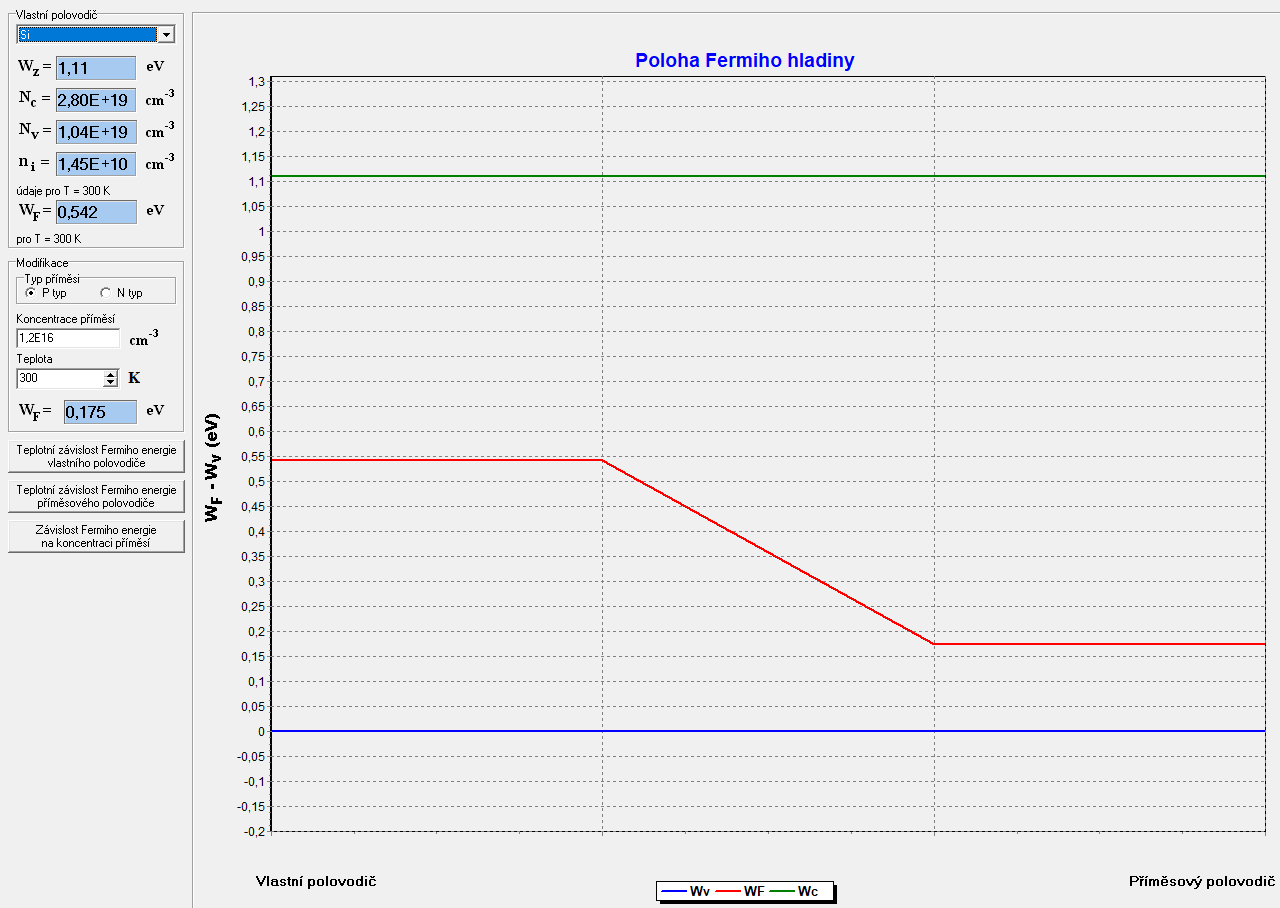
\includegraphics[width=\textwidth]{ukol1/si.png}
    % \end{minipage}
    % \hfill
    \begin{minipage}[t]{\textwidth}
        \begin{tikzpicture}
            \begin{axis}[
                width=\textwidth, 
                height=0.6\textwidth,
                title={srovnání šířky zakázaných pásu Si, Ge, InP a GaAs},
                xlabel={\(T\-[K]\)}, 
                ylabel={\(W\-[eV]\)},
                xmin=0, xmax=600,
                ymin=-0.1, ymax=1.5,
                % xtick={1000},
                ytick={0,0.1,...,1.5},
                legend pos=north west,
                ]
            \addplot[
                color=blue,
                ]
                coordinates {
                    (0   ,0)
                    (600 ,0)
                    };
                    \addlegendentry{\scriptsize \(W_v\)}
                    \addplot[
                        color=color-ge1,
                        ]
                coordinates {
                    (0   ,0.67)
                    (150 ,0.67)
                };
            \addlegendentry{\scriptsize \(W_{c-Ge}\)}
            \addplot[
                color=color-ge2,
                thick,
                domain=0:150,
                samples=500,
                %   color=red,
                %   mark=x,
                ]
                {0.335-x*2.369966297361443*10^(-5)};
                \addlegendentry{\scriptsize \(W_{F-Ge}\)}
                \addplot[
                    color=color-si1,
                ]
                coordinates {
                    (150 ,1.11)
                    (300 ,1.11)
                };
                \addlegendentry{\scriptsize \(W_{c-si}\)}
            \addplot[
                color=color-si2,
                thick,
                domain=150:300,
                samples=500,
                %   color=red,
                %   mark=x,
                ]
                {0.555-x*2.369966297361443*10^(-5)};
                \addlegendentry{\scriptsize \(W_{F-si}\)}
            \addplot[
                color=color-inp1,
                ]
                coordinates {
                    (300 ,1.344)
                    (450 ,1.344)
                };
            \addlegendentry{\scriptsize \(W_{c-InP}\)}
            \addplot[
                color=color-inp2,
                thick,
                domain=300:450,
                samples=500,
                %   color=red,
                %   mark=x,
                ]
                {0.672-x*2.369966297361443*10^(-5)};
                \addlegendentry{\scriptsize \(W_{F-InP}\)}
            \addplot[
                color=color-geas1,
                ]
                coordinates {
                    (450 ,1.4)
                    (600 ,1.4)
            };
            \addlegendentry{\scriptsize \(W_{c-GeAs}\)}
            \addplot[
                color=color-geas2,
                thick,
                domain=450:600,
                samples=500,
                %   color=red,
                %   mark=x,
                ]
                {0.7-x*2.369966297361443*10^(-5)};
            \addlegendentry{\scriptsize \(W_{F-GeAs}\)}
            \addplot[
                dotted,
                thick,
                color=color-geas2,
                domain=0:600,
                samples=500,
            %   color=red,
            %   mark=x,
                ]
                {0.7-x*2.369966297361443*10^(-5)};
            \addplot[
                dotted,
                color=color-inp2,
                domain=0:600,
                samples=500,
            %   color=red,
            %   mark=x,
                ]
                {0.672-x*2.369966297361443*10^(-5)};
            \addplot[
                dotted,
                color=color-si2,
                domain=0:600,
                samples=500,
            %   color=red,
            %   mark=x,
                ]
                {0.555-x*6.836964902*10^(-24)};
            \addplot[
                dotted,
                color=color-ge2,
                domain=0:600,
                samples=500,
            %   color=red,
            %   mark=x,
                ]
                {0.335-x*2.369966297361443*10^(-5)};
            \end{axis}
        \end{tikzpicture}
    \end{minipage}
\end{figure}
Nejtenší zakázaný pás ze skupiny \(A^{III}B^{V}\) má Indium antimonide \(InSb\), \(W_g = 0.17\-[eV]\) a naopak nejširší má Nitrid boru \(BN\), \(W_g = 6.36\) (příklad polovodiče, který by podle šířky zakázaného pásu měl být izolant a přesto se řadí mezi polovodiče).
Graf zároveň zobrazuje i závislost polohy Fermiho hladiny na Teplotě a je vidět, že se s měnící teplotou mění jen velmi málo. 

\begin{figure}[H]
    \begin{minipage}[t]{0.48\textwidth}
        \vspace{-70mm}
        \includegraphics[width=\textwidth]{ukol2/Ge.png}
    \end{minipage}
    \hfill
    \begin{minipage}[t]{0.52\textwidth}
        \begin{tikzpicture}
            \begin{axis}[
                    width=\textwidth, 
                    height=0.8\textwidth,
                    % title={},
                    xlabel={\(T\-[K]\)}, 
                    ylabel={\(W\-[eV]\)},
                    xmin=0, xmax=600,
                    ymin=-0.1, ymax=0.7,
                    ytick={-0.1,0,...,0.7},
                    legend pos=north west,
                ]
                \addplot[
                    color = red,
                    domain=0:600,
                    samples=500,
                ]
                {0.335-x*2.369966297361443*10^(-5)};
                \addlegendentry{\scriptsize \(W_F\)}
                \addplot[
                    color=blue,
                    ]
                    coordinates {
                        (0   ,0)
                        (600 ,0)
                    };
                \addlegendentry{\scriptsize \(W_v\)}
                \addplot[
                    color=green,
                    ]
                    coordinates {
                    (0   ,0.67)
                    (600 ,0.67)
                    };
                    \addlegendentry{\scriptsize \(W_c\)}
                \addplot[
                    dotted,
                    color = sedak,
                    domain=0:600,
                    samples=500,
                    ]
                    {0.335};
                \addplot[
                    dotted,
                    color = sedak,
                    domain=0:600,
                    samples=500,
                    ]
                    {0.32078020221583137};
            \end{axis}
        \end{tikzpicture}
    \end{minipage}
\end{figure}



\begin{figure}[H]
    \subsection*{Závislost polohy Fermiho hladiny na množství příměsí pro Ge}
    \(N_i = 1.40\cdot10^{13}\-[cm^{-3}]\); \(W_F = 0.67\-[eV]\); \(T = 300\-[K]\); \(W_i = 0.32789\-[eV]\)
    \begin{minipage}[t]{0.48\textwidth}
        \vspace{-70mm}
        \includegraphics[width=\textwidth]{ukol3/Ge.png}
    \end{minipage}
    \hfill
    \begin{minipage}[t]{0.52\textwidth}
        \begin{tikzpicture}
            \begin{semilogxaxis}[
                    width=\textwidth, 
                    height=0.8\textwidth,
                    % title={},
                    xlabel={\(p\-[cm^{-3}]\)}, 
                    ylabel={\(W\-[eV]\)},
                    xmin=10^14, xmax=10^24,
                    ymin=-0.6, ymax=1,
                    ytick={-0.6,-0.5,...,1},
                    legend pos=north west,
                ]
                \addplot[
                    color = red,
                    domain=10^14:10^24,
                    samples=10,
                ]
                {0.32789010110791567-0.025851999786000005*ln(x/(2.4*10^13))};
                \addlegendentry{\scriptsize \(W_F\)}
                \addplot[
                    color=blue,
                    ]
                    coordinates {
                        (10^14 ,0)
                        (10^24 ,0)
                    };
                \addlegendentry{\scriptsize \(W_v\)}
                \addplot[
                    color=green,
                    ]
                    coordinates {
                        (10^14 ,0.67)
                        (10^24 ,0.67)
                    };
                \addlegendentry{\scriptsize \(W_c\)}
                \addplot[
                    color=sedak,
                    ]
                    coordinates {
                        (10^14 ,0.32789010110791567)
                        (10^24 ,0.32789010110791567)
                    };
                \addlegendentry{\scriptsize \(W_i\)}
            \end{semilogxaxis}
        \end{tikzpicture}
    \end{minipage}
\end{figure}

\begin{figure}[H]
    \subsection*{Závislost polohy Fermiho hladiny na množství příměsí pro Si}
    \(N_i = 1.45\cdot10^{10}\-[cm^{-3}]\); \(W_F = 1.11\-[eV]\); \(T = 300\-[K]\); \(W_i = 0.54789\-[eV]\)
    \begin{minipage}[t]{0.48\textwidth}
        \vspace{-70mm}
        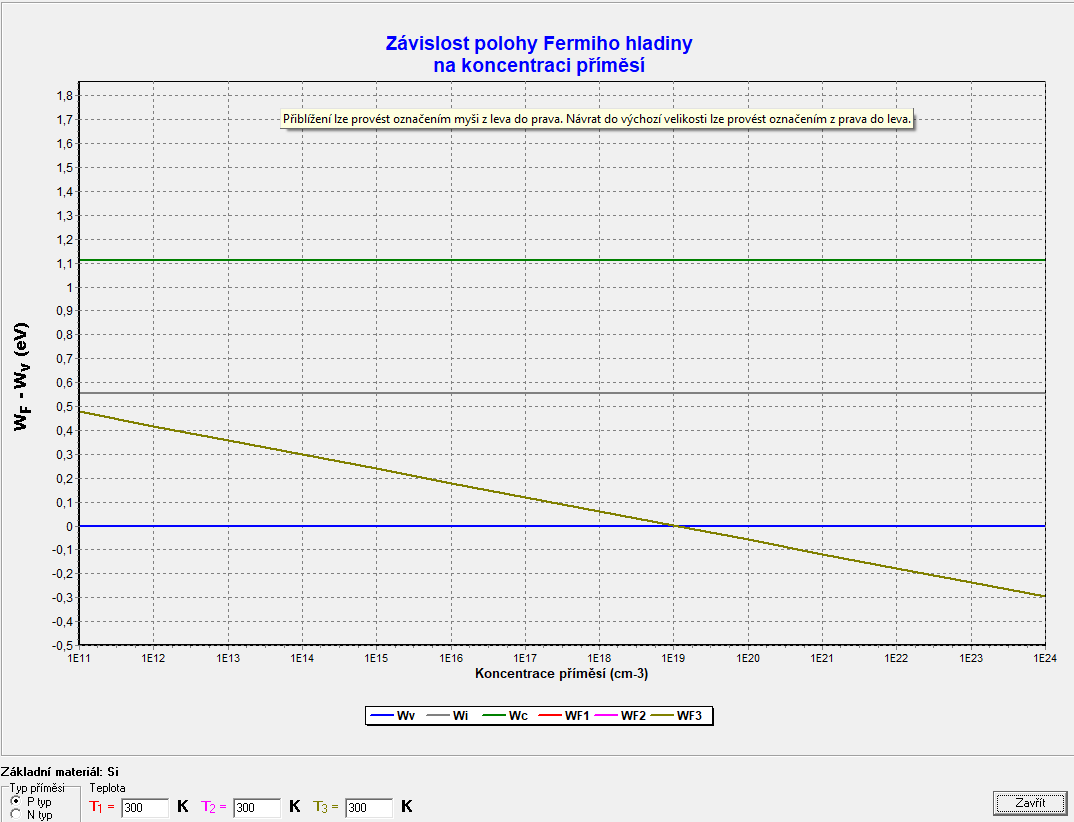
\includegraphics[width=\textwidth]{ukol3/si.png}
    \end{minipage}
    \hfill
    \begin{minipage}[t]{0.52\textwidth}
        \begin{tikzpicture}
            \begin{semilogxaxis}[
                    width=\textwidth, 
                    height=0.8\textwidth,
                    % title={},
                    xlabel={\(p\-[cm^{-3}]\)}, 
                    ylabel={\(W\-[eV]\)},
                    xmin=10^11, xmax=10^24,
                    ymin=-0.6, ymax=1.3,
                    ytick={-0.6,-0.5,...,1.3},
                    legend pos=north west,
                ]
                \addplot[
                    color = red,
                    domain=10^11:10^24,
                    samples=10,
                ]
                {0.5478901011079157-0.025851999786000005*ln(x/(1.45*10^10))};
                \addlegendentry{\scriptsize \(W_F\)}
                \addplot[
                    color=blue,
                    ]
                    coordinates {
                        (10^11 ,0)
                        (10^24 ,0)
                    };
                \addlegendentry{\scriptsize \(W_v\)}
                \addplot[
                    color=green,
                    ]
                    coordinates {
                        (10^11 ,1.11)
                        (10^24 ,1.11)
                    };
                \addlegendentry{\scriptsize \(W_c\)}
                \addplot[
                    color=sedak,
                    ]
                    coordinates {
                        (10^11 ,0.5478901011079157)
                        (10^24 ,0.5478901011079157)
                    };
                \addlegendentry{\scriptsize \(W_i\)}
            \end{semilogxaxis}
        \end{tikzpicture}
    \end{minipage}
\end{figure}

\subsection*{Závěr}
Teoretické vztahy velmi dobře odpovídají simulaci.
Pro výpočet Fermiho hladiny u příměsového polovodiče však uvedený vztah platí jen pro velké koncentrace příměsí.
Ze vztahu částečně i z grafů je vidět, že při dosazení koncentrace nižší než je hodnota \(n_i\), by příměs ovlivňovala Fermiho hladinu opačným směrem a při dosazení nulové koncentrace by měla být dokonce nekonečně velká resp. malá.

\end{document}